\chapter[Beethoven's Eleven Bagatelles, Op. 119, No. 1]{Ludwig van Beethoven - \textit{Eleven Bagatelles,} Op. 119, No. 1 (1803)}\label{chapter:beethoven}

Ludwig van Beethoven (1770-1827) was a composer who rose to prominence towards the end of the Classical period. He was born in Bonn, in Northwest Germany, where both his father and grandfather were court musicians in Cologne. His works have been divided into three periods: his birth until approximately 1802, from 1803-1814, and finally from 1815 to his death in 1827 \autocite{Kerman_Tyson_Burnham_Johnson_Drabkin_2001}, reflecting stylistic changes and important life events. In the first period, Beethoven mastered the popular genres and musical concepts of his time and crafting his style. He studied with Joseph Haydn (another Classical era composer), and Johann Georg Albrechtsberger, learning the art of counterpoint. This led to compositions of wide-use, including virtuosic works and pieces for beginner piano students\autocite{Burkholder_Grout_Palisca_2014}, and private works for connoisseurs and public symphonies. Then in 1802, Beethoven experienced a gradual loss of hearing, which would render him fully deaf in a few years. With the support from patrons and sales to publishers, he was able to compose works of a new depth, reflected by the struggles he was facing in life. Finally, in the third period, his music became more introspective and difficult for performers to play and listeners to comprehend\autocite{Kerman_Tyson_Burnham_Johnson_Drabkin_2001}. By 1818, his hearing had worsened to near-deafness, and this prompted another change in style. This period featured a higher degree of contrast than before \autocite{Burkholder_Grout_Palisca_2014}, and exaggerated. There was contrast between style, figuration, meter, and tempo. To balance the contrasts, there was also an emphasis on continuity, blurring divisions between phrases or movements.

The bagatelle form is a short piece of music, sometimes defined to literally be \say{something short, a trifle}, and is composed to be light-hearted\autocite{Brown_2001}. The title \say{bagatelle} itself does not imply any specific musical form, and the term has been used as a generic title since Beethoven's three sets of bagatelles for piano (Opus 33, 119, and 126). His later two sets of bagatelles (Opus 119 and Opus 126) are anything but simple and a trifle. These two sets reflect the introspective second period of Beethoven, as his hearing declined. 

\section{Bagatelle, Op. 119, No. 1}
The first of the bagatelles in Beethoven's Opus 119, this bagatelle is in ternary form, a three-part musical form, typically notated as \textit{ABA`}. The final section, \textit{A`}, is a repeat of the first \textit{A} section. Each section of the form is self-contained, usually closing in its own key\autocite{Tucker_Cochrane_2011}. Thus, the A section will close in the tonic key, and the A` section will modulate to another, related key, and closes in that key.\footnote{This key will typically be the dominant or relative major key of the one in the first A section.} The middle section, the \textit{B} section of a ternary piece, will provide a strong contrast to the two \textit{A} sections which surround it, contrasting both in theme and tonality.

The first section of the Bagatelle, the \textit{A} section, begins with a theme which sounds light and bouncy, but has a more subdued tonality. In the first four bars of this section, the articulation is hard to miss, as in Figure \ref{fig:beethoven-first-a-section-structure}\autocite{Henle_1978}. The first immediate element the performer will notice is the usage of articulation, specifically staccato. This gives the beginning of the movement a very bouncy character, juxtaposed with the otherwise mysterious nature of the A section. Beethoven also employs the use of phrase functions and phrase ends, which help a performer treat what the piece \say{says} in the style of the composer. Rests, as a form of articulation, are carefully placed throughout the A section. This causes the performer to ensure that they pause at appropriate times through the piece. 

\begin{figure}[h]
	\centering
	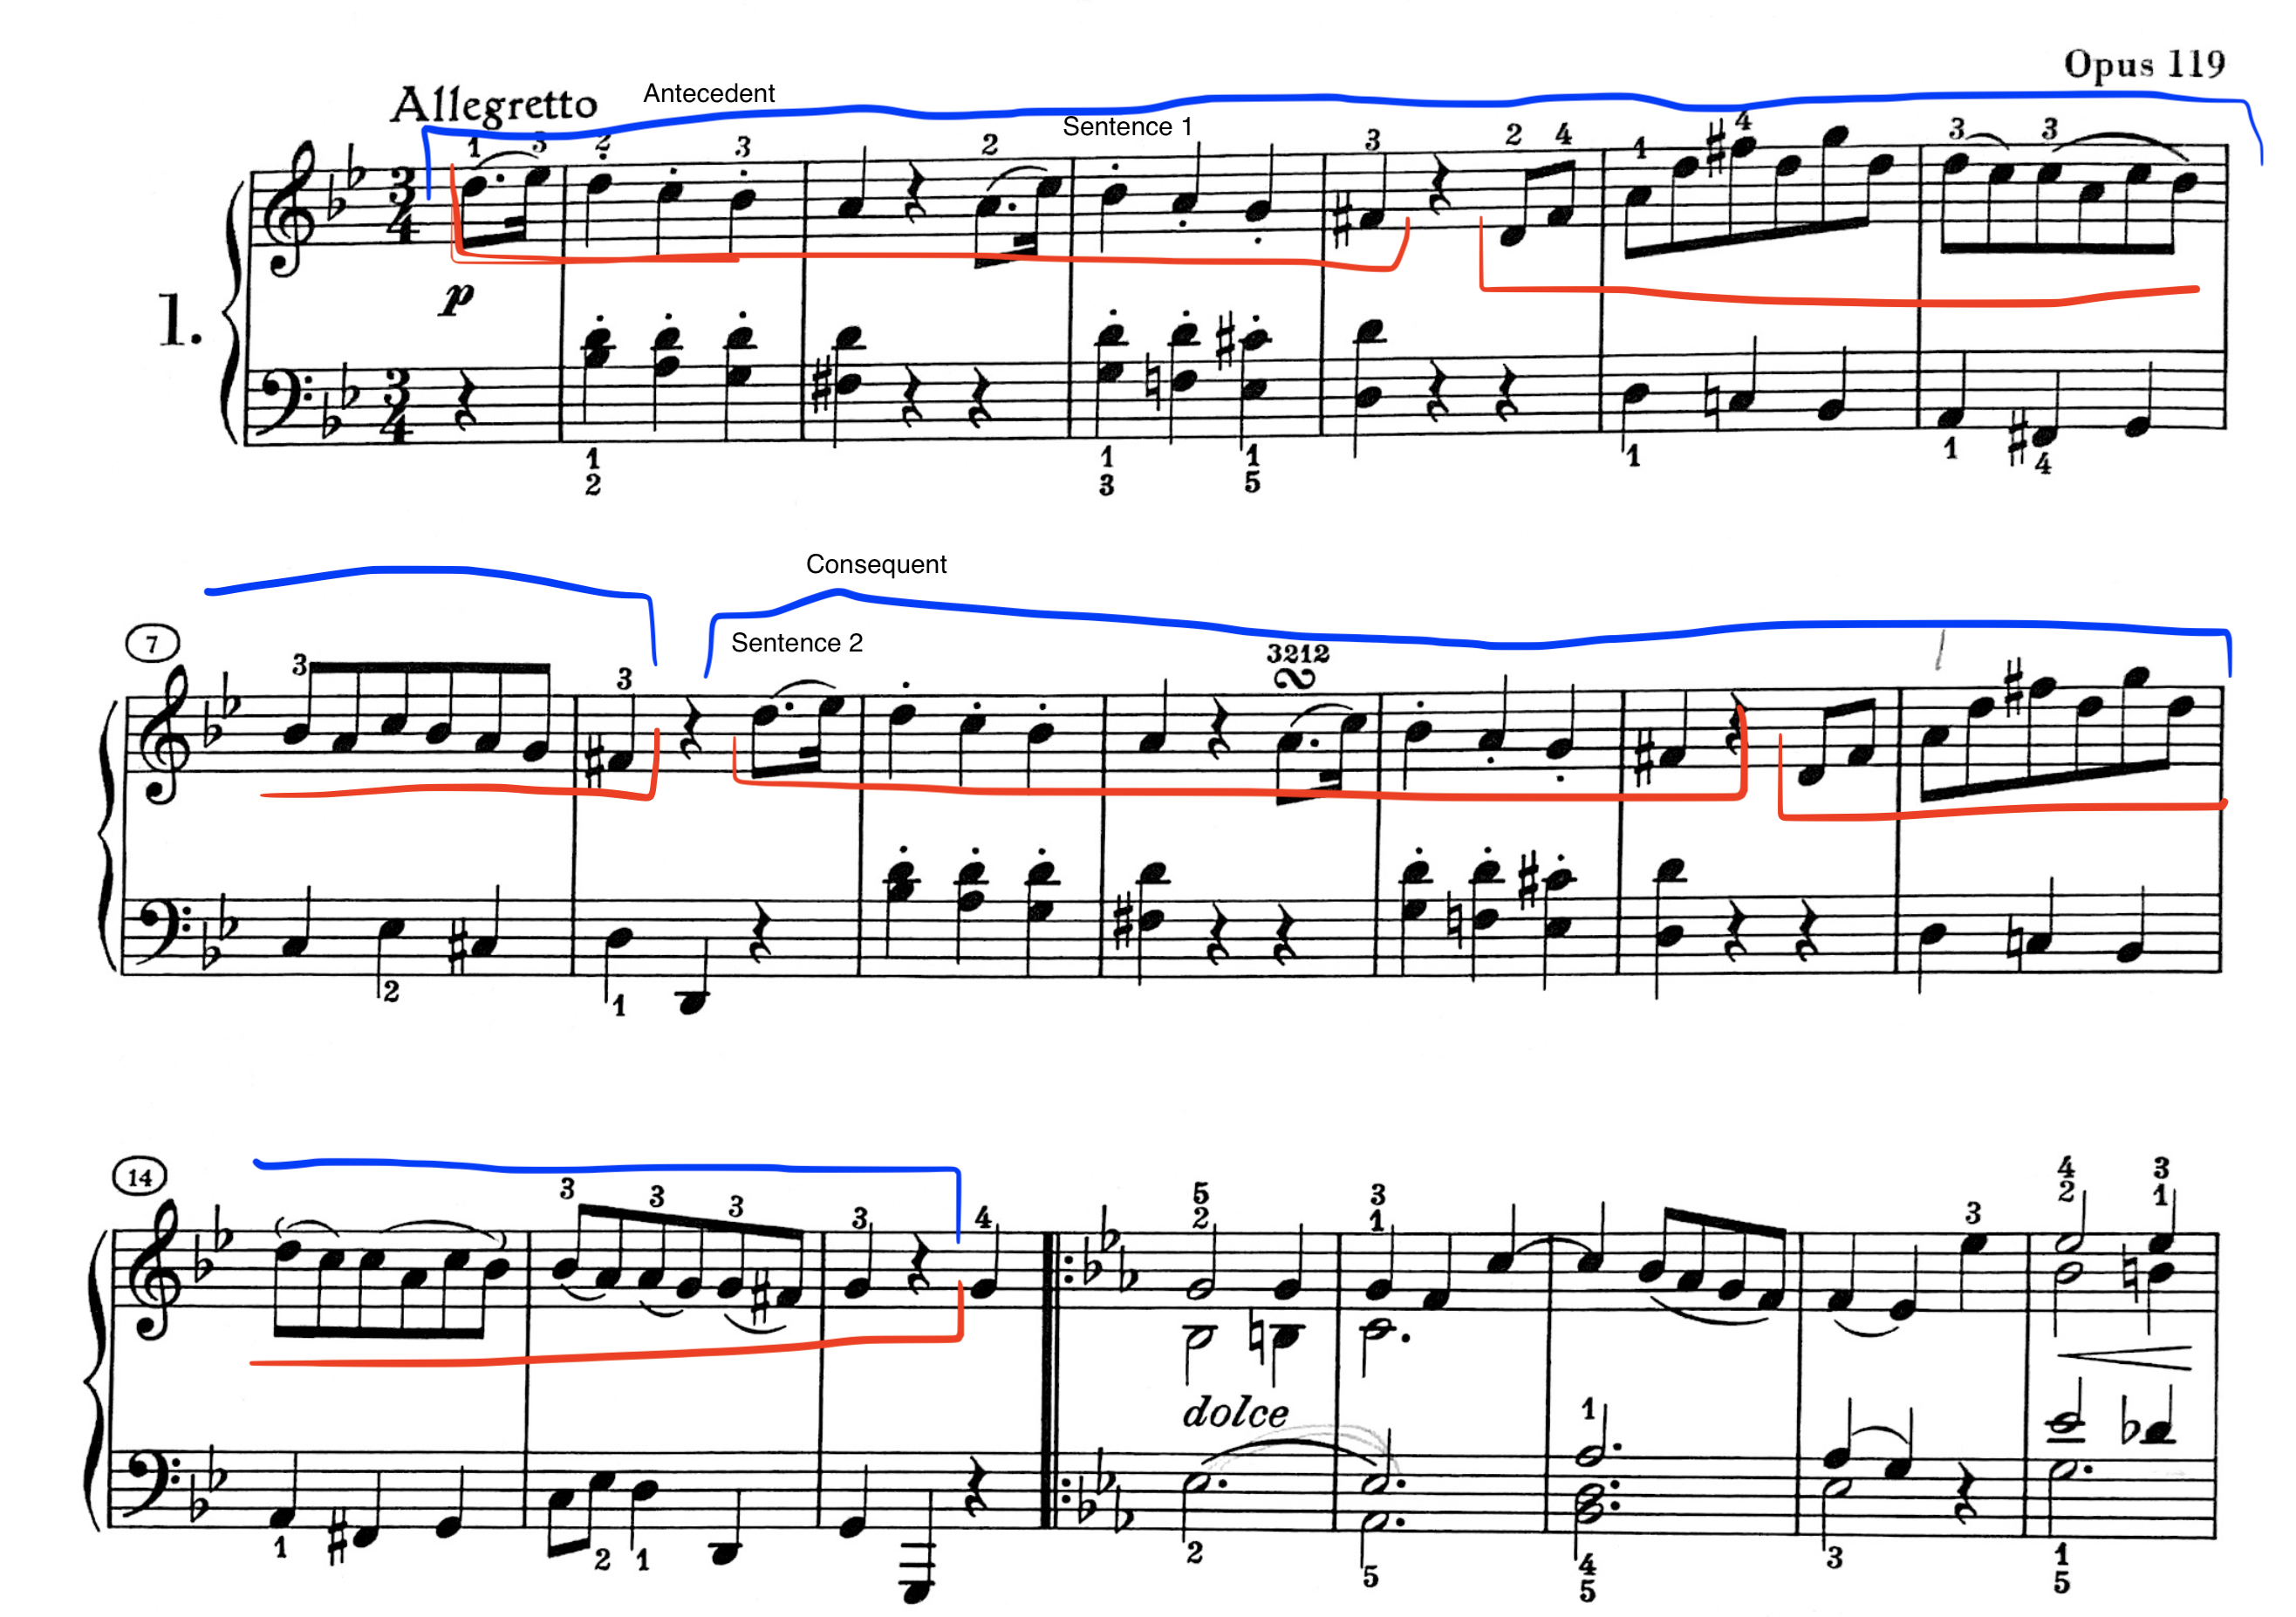
\includegraphics[width=0.5\textwidth]{figures/beethoven-first-a-section-structure.jpg}
	\caption{Ludwig van Beethoven, Eleven Bagatelles, mm. 1-21}
	\label{fig:beethoven-first-a-section-structure}
\end{figure}

In the first eight bars of the A section, as seen in Figure \ref{fig:beethoven-first-a-section-structure}\autocite{Henle_1978} and demarcated in red brackets, can clearly be broken into several parts. The first four measures of the section, as in Figure \ref{fig:beethoven-first-a-section-structure}\autocite{Henle_1978}, are a repeat of each other. Bars 3-4 repeat bars 1-2, but are only a minor third interval lower. The two parts which make up the A section are marked with the use of a quarter rest in between, in bar 4. This second half of the section's first eight bars, what will be known as the \say{continuation,} is to give the listener the feeling that there is an ending coming \autocite{Kerman_Tyson_Burnham_Johnson_Drabkin_2001}. This ending is normally signified by the use of quicker rhythms and an increase in harmonies. Finally, in bar 8 this sensed ending appears, but not in an expected way. Bar 8 contains a half-cadence, a type of cadence\footnote{A cadence can be defined as a melodic or harmonic motion, which is typically associated with the ending of a phrase, section, movement, or composition.}\autocite{Nagley_Whittall_2011} which ends the phrase on a dominant chord, here being the chord D Major. So, the phrase ends with unresolved harmonic tension, and implies that another phrase will follow it.

Bar 9 of the section, as in Figure \ref{fig:beethoven-first-a-section-bars-nine-to-sixteen}\autocite{Henle_1978} and bracketed in red, is an exact repeat of bar 1. Thus, there is a larger organizational structure to this piece, and the first A section, than the first eight bars of the section.\footnote{These first eight bars of the A section form a sentence. A sentence in music is defined as a complete musical idea, such as a self-contained theme, which is the sum or two or four phrases arranged in a complementary manner.} As bars 1-8 are almost repeated exactly in bars 9-16, albeit not immediately, this signals the structure known as a period. A period is similar to a sentence; it has two parts: the antecedent and the consequent, which are bracketed in blue in Figure \ref{fig:beethoven-first-a-section-structure}\autocite{Henle_1978}. Each section starts exactly the same, but end differently. The antecedent phrase sets up the musical idea that will be treated during the period, and ends on a weak type of cadence, including the half-cadence, or deceptive cadence. The consequent phrase, which follows the antecedence, repeats the idea found in the antecedent phrase, and ends with a stronger cadence (such as the perfect authentic cadence, or PAC), signifying the end of a phrase. The repeat of material first found in bar 1-9 signals to the performer that there is a period. There is a half-cadence in bar 8, as in Figure \ref{fig:beethoven-first-a-section-hc}\autocite{Henle_1978}, which is a weak cadence. Then, bars 9-16 contain material that is repeated. In bar 16, instead of a half-cadence ending the phrase, there is a PAC, ending the phrase in the tonic key. As seen in Figure \ref{fig:beethoven-first-a-section-structure}\autocite{Henle_1978}, the period which makes up the first A section is a nested period, in that in the period itself, there are two sentences nested inside. The section will come back in the end of the piece, in the \textit{A`} section. 

\begin{figure}[h]
  \centering
  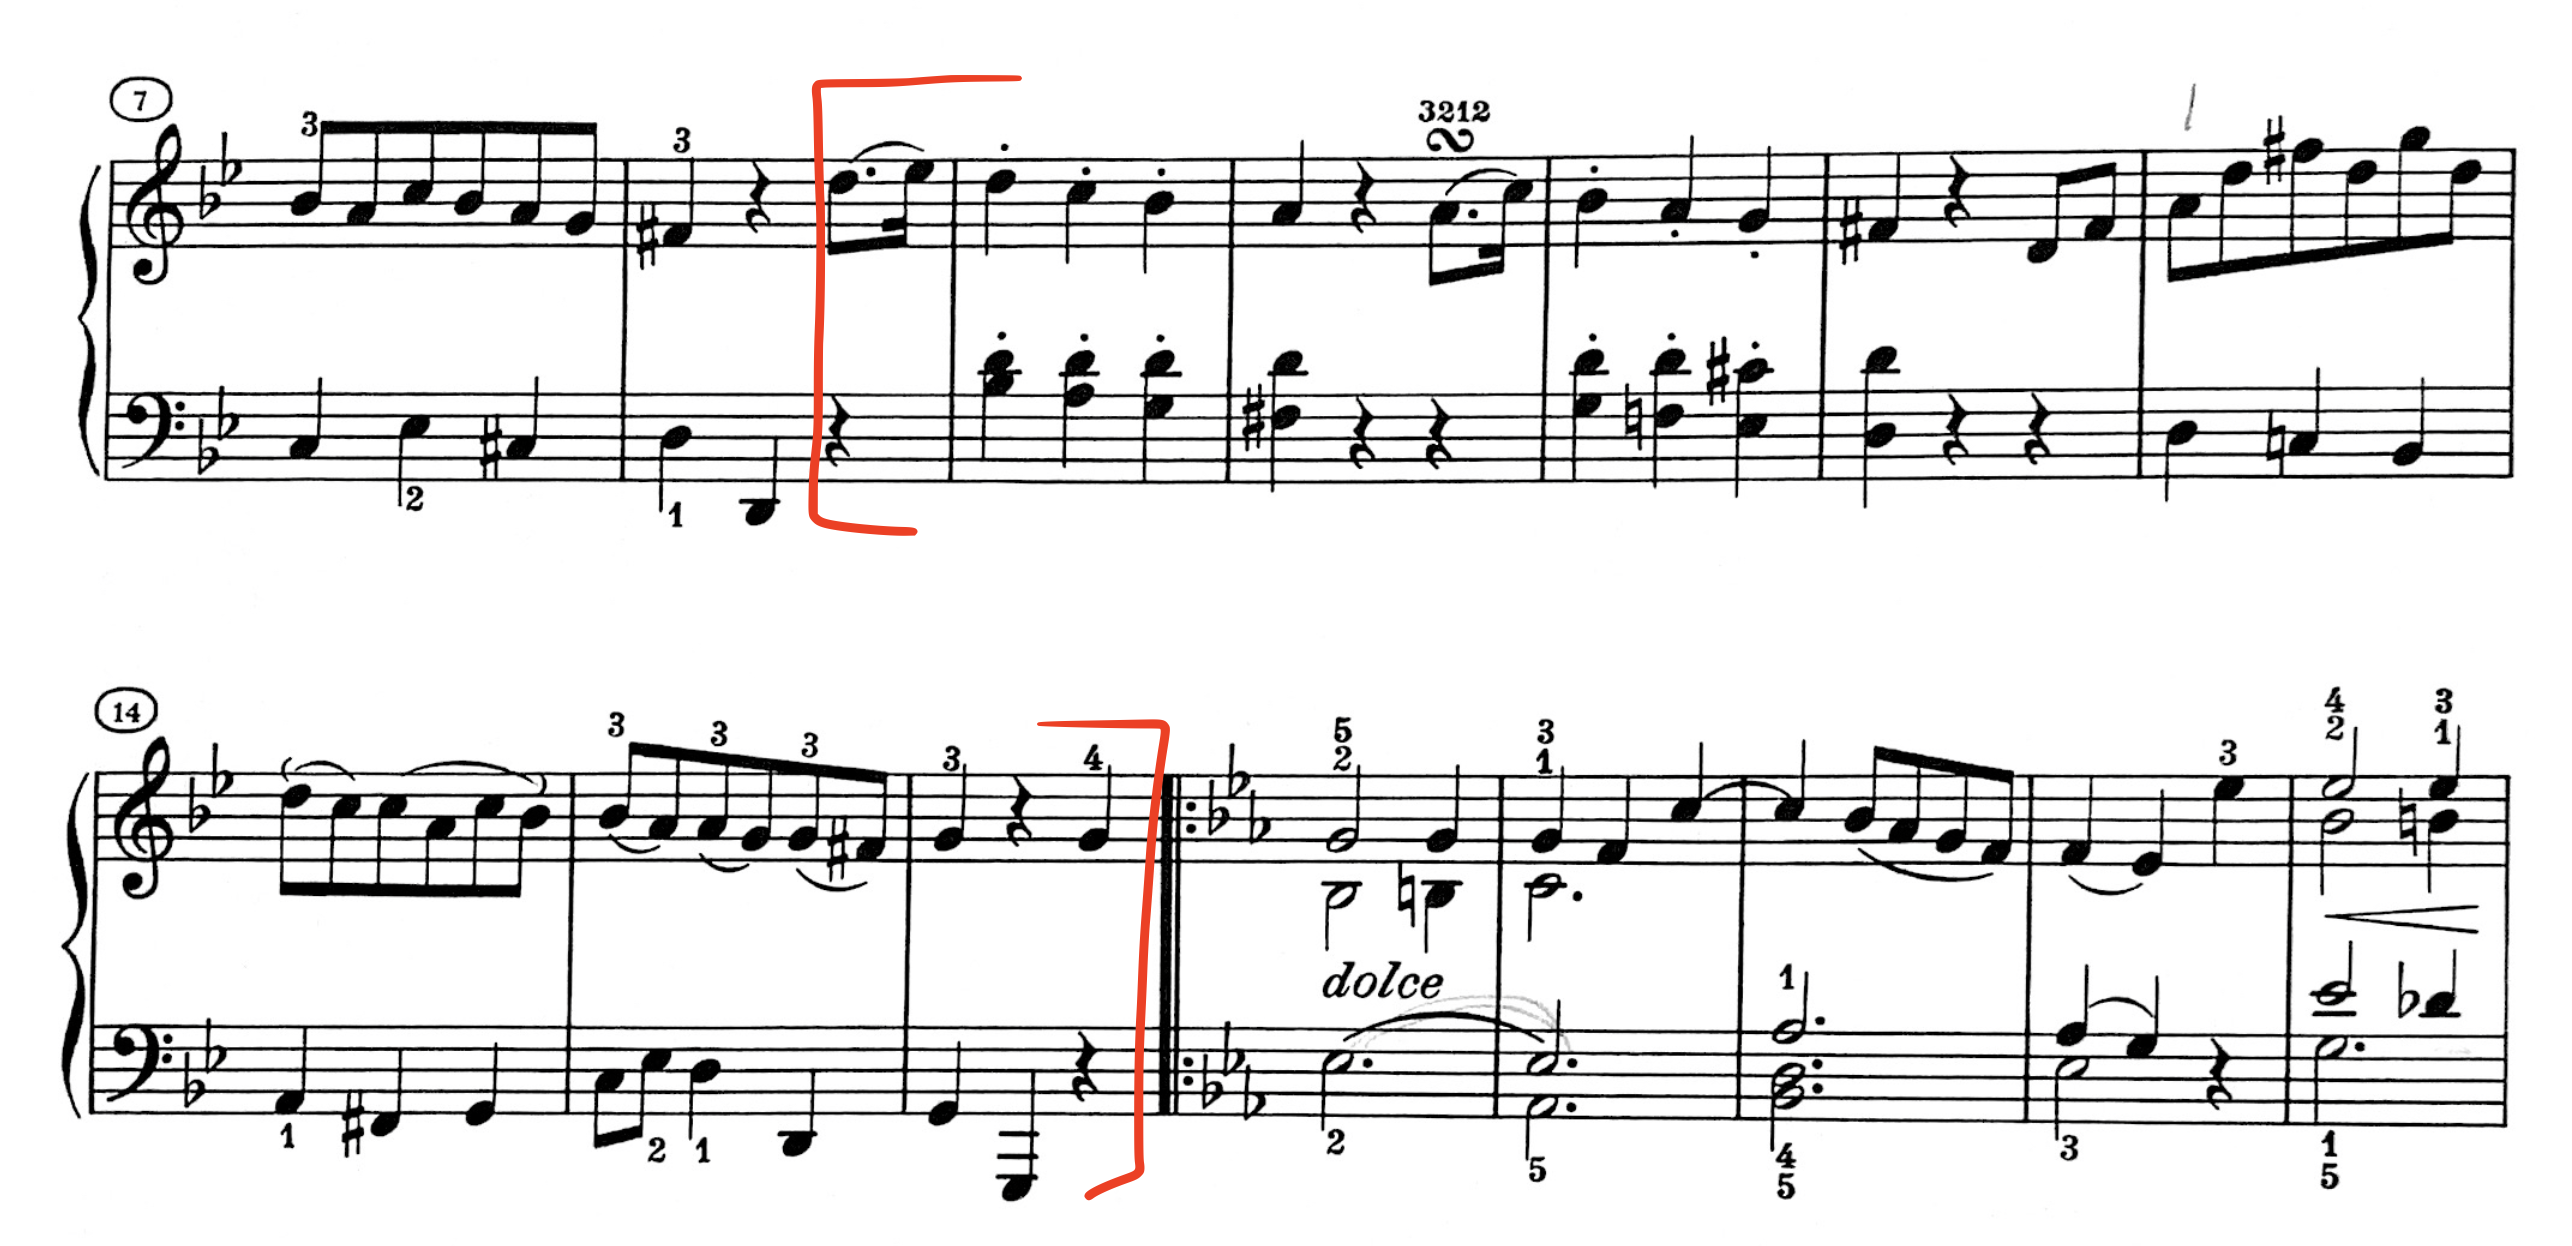
\includegraphics[width=\textwidth]{figures/beethoven-first-a-section-bars-nine-to-sixteen.jpg}
  \caption{Ludwig van Beethoven, Eleven Bagatelles, mm. 7-21}
  \label{fig:beethoven-first-a-section-bars-nine-to-sixteen}
\end{figure}

\begin{figure}[h]
	\centering
	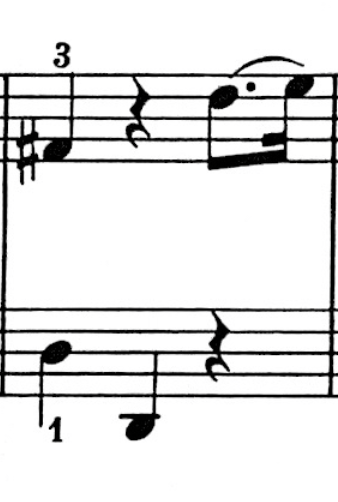
\includegraphics[width=0.4\textwidth]{figures/beethoven-first-a-section-hc.jpg}
	\caption{Ludwig van Beethoven, Eleven Bagatelles, mm. 7-8}
	\label{fig:beethoven-first-a-section-hc}
\end{figure}

As previously mentioned, in the ternary form, each section--the A, B, and A`--is able to stand on its own. The B section will provide a strong contrast with the A and A` sections which surround it, in theme and tone. For this B section, Beethoven modulates to the key E\musFlat{} Major. The sudden key change from G Minor to related key E\musFlat{} Major alerts listeners to understand that this is a new section. Other differences in the B section from the first A section include a difference in the section's articulation and harmony. With articulation, as seen in Figure \ref{fig:beethoven-b-section}\autocite{Henle_1978} and bracketed in red, there are no staccatos in this section. Instead, the section flows together more than the A section. It sound much more lyrical, and connected. Opposed to the left-hand in the A section, the B section's left-hand plays more block chords, and this leads to an overall greater depth in the section's sound. These left-hand notes are also played in a lower octave than the notes that were played in the A section.

\begin{figure}[h]
	\centering
	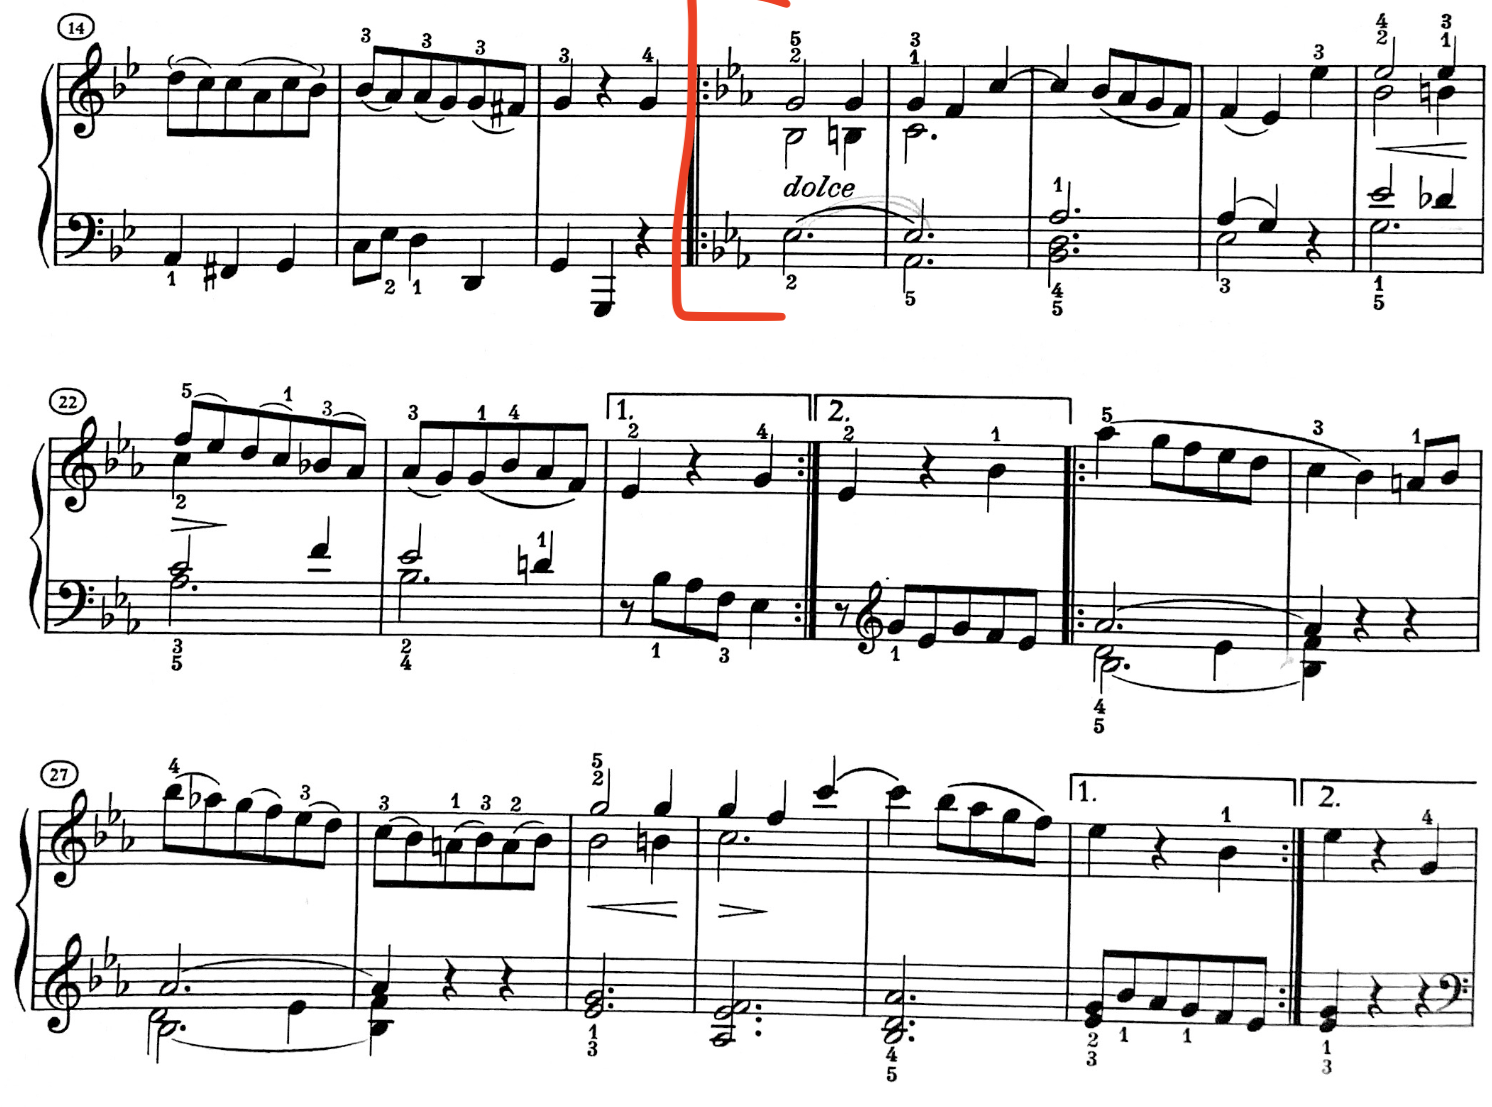
\includegraphics[width=0.5\textwidth]{figures/beethoven-b-section.jpg}
	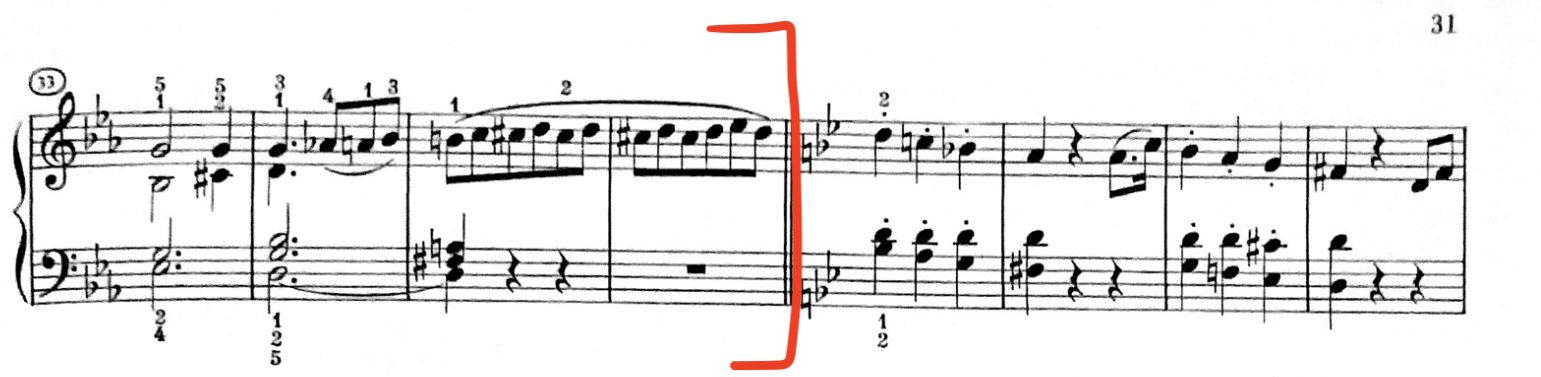
\includegraphics[width=0.5\textwidth]{figures/beethoven-b-section-part-two.jpg}
	\caption{Ludwig van Beethoven, Eleven Bagatelles, mm. 14-40}
	\label{fig:beethoven-b-section}
\end{figure}

In bar 37, there is a return to the material which appeared in the A section. This marks the A` section. However, instead of being a strict restatement of all the material of the first A section, Beethoven repeats the material with variation. This is defined as a phrase of music which is a varied version of an original theme. Some variations may follow this original theme very closely, and others may be more original, only referencing the original theme through harmonies or melodic references.\autocite{Kennedy_Kennedy_Rutherford-Johnson_2013b} In the A` section, while there a return to the material that was introduced in the first A section, the material is also now a variation. The first A section's melody is still intact, but it is now more \say{hidden}, with the melody notes sounding on every second eighth note, as seen in Figure \ref{fig:beethoven-a-prime-melody-variation}\autocite{Henle_1978}. Beginning in beat three of bar 44, the melody sounds on every second eighth note. The shape and melody of the original A section is still there, only less obvious.

\begin{figure}[h]
	\centering
	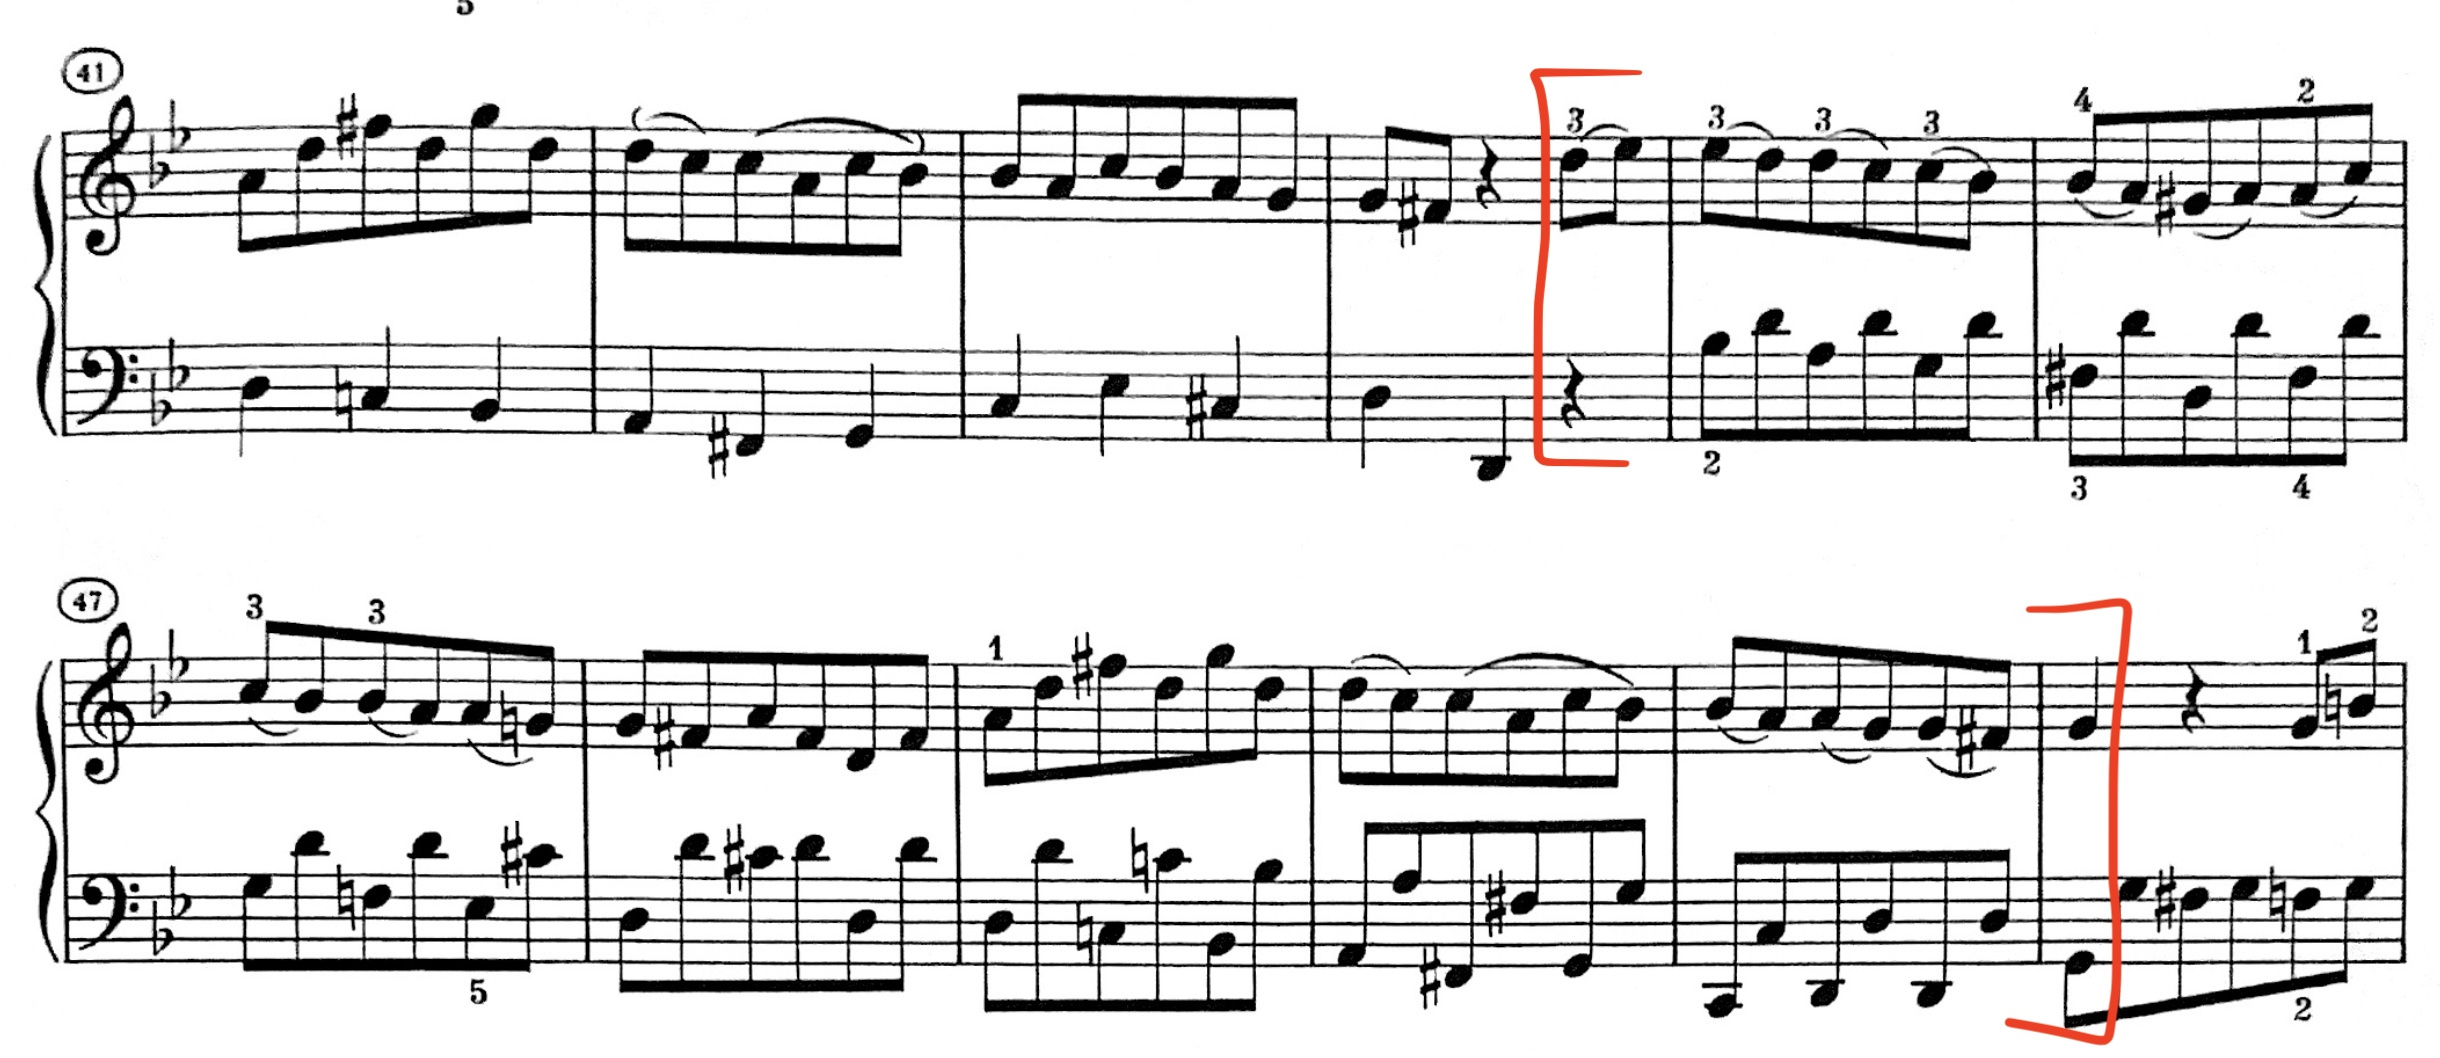
\includegraphics[width=\textwidth]{figures/beethoven-a-prime-melody-variation}
	\caption{Ludwig van Beethoven, Eleven Bagatelles, mm. 41-52}
	\label{fig:beethoven-a-prime-melody-variation}
\end{figure}

\subsection{A Trifle}

This piece is in ternary form, and so has three different ``characters'' that must receive different treatments for their thematic material. The first section, the A section, is light and bouncy in sound, and employs staccato and other phrasing tools to create it. Notes are clearly marked as either staccato or legato, and notes that have neither a staccato or legato marking are meant to be played \textit{detaché} (or detached, a halfway point between legato and staccato). Quarter rests are also scattered through the A section, which serve as another point of articulation. This allows my performance to pause at the appropriate times that Beethoven had written into the music, and gives the section the bouncy flow to which it is intended. Later, in the second half of the A section (bars 9-16) in Figure \ref{fig:beethoven-first-a-section-bars-nine-to-sixteen}\autocite{Henle_1978}, there are also noticeable two-note slurred eighth note phrases and turns which add ornamental lightness to the section. Bar 9 contains a turn placed on the note A which, as a performer, indicates that I must play the notes A, B, A, C in that order, ``turning'' over the note B to get to C. This turn, and the others like it which reappear in the A' section also add to bouncy upbeat feeling. In addition, the period previously mentioned also adds to a flowy and bouncy character. There is a half-cadence in bar 8 of Figure \ref{fig:beethoven-first-a-section-hc}\autocite{Henle_1978} which is a weak cadence. I play this to indicate to the listener that there is still more of the section left to play, but without letting go of the built-up tension so far in the section. The half-cadence does not have the same finality as the PAC (in Figure \ref{fig:beethoven-first-a-section-structure}\autocite{Henle_1978}), which is able to signify the end of a phrase. Thus, in the second half of the A section, as I approach the PAC, I do not indicate to the listener early that we are approaching the end of a phrase. Instead, I continue playing as I did in the first half of the A section, and only end the phrase with finality in bar 16. 

Then, the B section is noticeably calmer than the A section, in which the material treated is much smoother and played legato. As it sounds much more lyrical and connected, there is a greater depth to the texture, which was not present in the A section. There are no staccato markings within the B section, but many half notes, notes played legato, and moving eighth notes, grouped into twos or fours. The left-hand contains many of the half notes played in this section, so the primary motions in the section are in the right-hand, which contains a combination of half notes, quarter notes, and eighth notes, all played legato. As the B section begins, I take note of the \textit{dolce} (``sweet'') expressive marking. This section is meant to be played sweetly, as indicated by the numerous legato markings, and so I do so. In contrast to the A section, the B section is played very warmly, with many dynamic contrasts and changes through the section. The right-hand in the B section begins to sing, akin to the ways in which a solo singer might sing a similar passage. Additionally, we notice that in the left-hand, the block chords are played roughly an octave lower than the left-hand plays in the A section. This also contributes to the warm feeling of the B section, as half the notes are below Middle C, allowing for the low bass notes to provide a warm and round sound to balance the singing in the right-hand. 

In measure 37, the A section returns, as A'. This section acts as a variation to the material that was treated in the first A section, and so the A' section contains more motion than the A section. Beginning in the last beat of bar 44, the second half of the material that was in the A section is altered and broken into eighth notes, grouped into sets of two. The melody that was found in the equivalent section of the A section is still found here in the A' section; however, the melody line sounds on every second eighth note, as in Figure \ref{fig:beethoven-a-prime-melody-variation}\autocite{Henle_1978}. It is here in which I add energy that was not in the A section. Though explicit dynamic markings are not found within the section, I increase the dynamic level from its baseline \textit{mezzo forte} to \textit{forte} when the right-hand's melody approaches its relative peak pitch, and play the dynamic level \textit{piano} when the melody line approaches its relative lowest pitch. This adds suspense closer to the ending of the song, especially in bar 50 of Figure \ref{fig:beethoven-a-prime-melody-variation}\autocite{Henle_1978}, in which the left-hand harmony line becomes lower in pitch, and the right-hand's melody line is rising in pitch. The left-hand adds depth and warmth, and so combined with the right-hand literally brings the phrase to a new height, as the dynamic level becomes \textit{forte}, then comes back down to a \textit{piano} on the brief half-cadence. From here, there is a phrase of moving eighth notes, along with dynamic markings to add energy in favor of the bouncy character of the A section. Here, there is depth to the moving eighth notes, which I continue to sound in a mixture of legato and staccato. 

